\documentclass[a4paper,fleqn]{cas-dc}

\usepackage[authoryear]{natbib}
\usepackage{amsmath}
\usepackage{amsfonts}
\usepackage{amssymb}
\usepackage{booktabs}
\usepackage{tikz}
\usetikzlibrary{shapes.geometric, arrows.meta, positioning, fit, backgrounds}

\begin{document}
\let\WriteBookmarks\relax
\def\floatpagepagefraction{1}
\def\textpagefraction{.001}

\shorttitle{Hierarchical Deep Learning for Carbonate Microfacies}
\shortauthors{M. Muradi et~al.}

\title[mode=title]{Deep learning-based classification of carbonate microfacies components in thin-section images}

\author[1]{Musawer Muradi}[orcid=0000-0001-0000-0000]
\cormark[1]
\ead{musavir.muradi@gmail.com}
\credit{Conceptualization, Methodology, Software, Writing -- Original Draft}

\author[2]{Arnaud Gallois}
\ead{arnaud.gallois@kocaeli.edu.tr}
\credit{Geological Interpretation, Data Curation}

\author[1]{Alev Mutlu}
\ead{alev.mutlu@kocaeli.edu.tr}
\credit{Data Curation, Writing -- Review \& Editing}

\affiliation[1]{organization={Department of Computer Engineering, Kocaeli University},
                city={Kocaeli},
                country={Turkiye}}

\affiliation[2]{organization={Department of Geological Engineering, Kocaeli University},
                city={Kocaeli},
                country={Turkiye}}

\cortext[cor1]{Corresponding author}

\begin{abstract}
Automated analysis of carbonate thin sections is fundamentally challenged by extreme class imbalance: structureless background grains such as peloids routinely make up more than 87\% of annotated samples, while the grain types that carry the most geological information --- broken ooids, intraclasts --- may account for less than 2\%. When standard deep networks are trained on distributions this skewed, they collapse into majority-class detectors, learning to predict ``peloid'' for nearly everything and achieving deceptively high accuracy while failing entirely on the classes that matter. This paper describes how encoding the established geological taxonomy of carbonate grains directly into the structure of a deep network can fundamentally change this behaviour.

The proposed architecture, a hierarchical ResNet-18 with three independent binary decision heads, decomposes the four-class problem into a sequence of binary questions that mirror the way a geologist would classify a grain: first, is this a peloid or not; if not, is it ooid-like or an intraclast; if ooid-like, is it intact or broken? Each head is trained with a stage-specific variant of Focal Loss, calibrated to the local class imbalance at that particular decision, and the rarest class --- broken ooids, present in fewer than one in a hundred grains --- is explicitly oversampled at 15 times its natural frequency within every training batch. Training follows a four-phase staged curriculum that prevents the peloid-dominated Stage~1 decision from monopolising the shared backbone, leaving the minority-class heads with a poorly adapted feature extractor. At inference time, each grain is classified six times under different geometric orientations and the predictions are averaged, reducing variance on the morphologically ambiguous boundary cases that the network finds hardest.

On a held-out test set of 529 grains, the full pipeline achieves a Balanced Accuracy --- the arithmetic mean of per-class recall, which weights each class equally regardless of how many samples it contains --- of 83.5\%, with an Overall Accuracy of 92.1\%. The ablation study reveals that without oversampling, the hierarchical architecture alone recovers only 16.7\% recall for broken ooids, close to random chance. Adding oversampling raises this to 66.7\%, and the staged training curriculum together with inference-time averaging brings the final result to 83.3\% recall for that class while simultaneously improving intraclast recall from 66.7\% to 71.4\%. A standard flat ResNet-18 trained with cross-entropy on the same data achieves a Balanced Accuracy of 86.9\% on this specific test split, a higher headline figure driven almost entirely by the fact that it correctly identifies all six broken ooid test instances by chance --- a result whose 95\% confidence interval spans [54\%--100\%] and is therefore not statistically reliable. The hierarchical model's more consistent advantage lies in intraclast recall, which it recovers to 71.4\% against the flat model's 61.9\%, illustrating that the architectural design produces a more balanced distribution of recall across all minority classes simultaneously rather than excelling on one at the expense of another.
\end{abstract}

\begin{highlights}
\item A hierarchical ResNet-18 encodes carbonate grain taxonomy into three sequential binary decisions, isolating minority-class heads from peloid-dominated gradients.
\item Without targeted oversampling, the hierarchical base model achieves only 16.7\% recall for broken ooids; the full pipeline raises this to 83.3\%.
\item The complete pipeline --- staged training, 15$\times$ oversampling, and inference-time augmentation --- achieves 83.5\% Balanced Accuracy and 92.1\% Overall Accuracy on a held-out test set of 529 grains.
\end{highlights}

\begin{keywords}
Carbonate Microfacies \sep Deep Learning \sep Class Imbalance \sep Hierarchical Classification \sep Focal Loss
\end{keywords}

\maketitle

\section{Introduction}

Automated petrographic analysis of carbonate rocks has attracted growing interest over the past decade, driven by the need to reduce the time and subjectivity inherent in manual grain-by-grain thin-section interpretation. Identifying grain types accurately matters not only because it is tedious to do by hand, but because the relative proportions of different grains carry direct information about the energy conditions under which a carbonate platform was deposited --- information used in groundwater aquifer modelling, hydrocarbon exploration, and palaeoenvironmental reconstruction. The grain types most informative for these purposes are, by their nature, rare: broken ooids, which indicate episodes of high-energy reworking such as storm or tidal events, may appear in fewer than one in every hundred grains in a typical thin section \citep{flugel2010}.

This rarity creates a fundamental problem for standard deep learning approaches. A network trained to minimise cross-entropy loss on a dataset where 87\% of samples belong to one class will find the globally optimal solution by predicting that class for almost every input. The result looks impressive on a raw accuracy metric --- an 87\% peloid rate gives an 87\% accuracy for free, without the network learning anything useful about the minority classes --- but it fails completely as a scientific tool, as the ablation results in Section~\ref{sec:results_ablation} directly confirm. This is not a minor calibration issue that can be solved by adjusting a single hyperparameter. It is a structural property of the loss landscape when class distributions are this extreme, and addressing it requires rethinking the architecture and the training procedure from the ground up.

The approach taken in this work starts from the observation that the geological classification of carbonate grains is not a flat four-way choice. It follows a branching taxonomy: a grain is first identified as either a peloid or something else; if it is not a peloid, the next question is whether it shows the concentric cortical fabric of an ooid-like grain or the angular, reworked texture of an intraclast; and if it is ooid-like, a final question resolves whether the cortex is intact or fractured. This hierarchical logic, which any trained sedimentologist would recognise, can be embedded directly into a neural network by replacing a single four-class output head with three successive binary decision heads, each responsible for one branch of the taxonomic tree. The consequence is that the head responsible for distinguishing whole from broken ooids --- the most data-starved and morphologically difficult decision --- is never exposed to peloid samples during its gradient updates. It learns only from ooid-like grains, in an environment where its signal is not overwhelmed.

The specific contributions of this paper are as follows. First, we introduce a hierarchical ResNet-18 architecture that encodes carbonate grain taxonomy as a sequence of three binary decisions, with each head receiving gradients only from the grain sub-population relevant to that decision. Second, we design a stage-wise Focal Loss scheme in which the class-balancing weight $\alpha$ is calibrated separately for each head to reflect the local class imbalance at that node of the decision tree. Third, we introduce a four-phase staged training curriculum that prevents the peloid-saturated Stage~1 head from monopolising the shared backbone's gradient signal during the critical early phase of training. Fourth, we demonstrate through a detailed ablation study that each of these components contributes measurably to minority-class recall, with targeted oversampling emerging as the single most important intervention: without it, the hierarchical base model recovers only 16.7\% of broken ooid instances on the test set.

\section{Literature Review \& Domain Challenges}

\subsection{The Bottleneck of Petrographic Data Collection}
A persistent challenge in computational geosciences is the acquisition of labelled data at sufficient scale and quality. Unlike natural image datasets, where non-expert annotators can reliably label thousands of images per day, petrographic labelling requires a trained sedimentologist who can interpret grain boundaries, textures, and diagenetic fabrics under a microscope. This creates a hard ceiling on dataset size that cannot be overcome simply by hiring more annotators \citep{koeshidayatullah2020}. Even when large datasets are assembled, the class distribution is constrained by geology: a single thin section from a high-energy carbonate environment may contain thousands of peloids but only a handful of broken ooids, so the imbalance does not diminish as more material is imaged from the same succession.

This scarcity of minority-class data has consequences that go beyond simple underfitting. \citet{dalhat2025} found that even across a reasonably large collection of 3,179 microscopic images spanning 40 mineral types, per-class accuracy varied dramatically, with the decisive discriminative signal coming from fine-grained textural cues at grain boundaries rather than gross morphological shape. In carbonate microfacies, the morphological overlap between classes is even more severe: a heavily micritised ooid and a structureless peloid may be visually indistinguishable to a network that has not seen enough of each to learn the subtle textural differences. More training data helps, but it cannot substitute for a training procedure that actively preserves the gradient signal from those rare, ambiguous examples.

\subsection{The Performance Gap Between Macroscopic and Microfacies Classification}
The majority of reported successes in geological image classification come from macroscopic rock typing, where the visual differences between classes --- granite versus sandstone, for example --- are large enough to be obvious even under relatively weak feature extractors. In this regime, fine-tuned ResNet or VGG architectures on ImageNet-pretrained weights routinely achieve accuracy above 95\%. \citet{chen2023} reported 99.1\% accuracy using a ResNet-34 backbone on seven macroscopic rock types, a figure that reflects how easy the underlying discrimination task is when classes are visually distinct.

Microfacies classification does not benefit from this separation. The grain types we are attempting to distinguish --- peloid, ooid, intraclast, and broken ooid --- share the same basic circular or sub-circular geometry and similar optical properties under plane-polarised light. The distinction between an intact ooid and a broken one relies on the presence of a jagged fracture plane through the cortical laminae, a feature that may occupy only a small portion of the grain boundary at the scale of a 96-pixel crop. The distinction between a peloid and a heavily diagenetically altered ooid may rest on the faintest residual trace of concentric lamination \citep{flugel2010}. These are not tasks where a pre-trained convolutional backbone can immediately transfer its knowledge; the relevant signal must be learned from a small and heavily imbalanced dataset.

\subsection{Related Work in Automated Carbonate Petrography}
\label{sec:lit_taxonnet}
Several groups have applied deep learning directly to carbonate thin-section classification, providing useful context for the difficulty of this task. \citet{pireslima2020} used fine-tuned convolutional neural networks to classify five microfacies types from the Sycamore Formation, achieving above 90\% accuracy when evaluated on samples from the same laboratory. When the same model was evaluated on samples from a different laboratory --- same rock type, different preparation and imaging conditions --- accuracy dropped to approximately 40\%. This collapse illustrates how fragile flat convolutional architectures can be when deployed outside their training distribution, a problem that only compounds when the training distribution is already dominated by a single class.

\citet{liu2020} circumvented this problem to some extent by assembling a dataset of over 30,000 images across 22 fossil and abiotic grain categories, large enough that even minority classes had several hundred training examples. Their Inception ResNet v2 model achieved 95\% top-one accuracy overall, but precision dropped to 0.88 for morphologically similar pairs such as bivalves and brachiopods, compared to above 0.99 for visually distinct categories. The implication is that even at this scale, inter-class morphological overlap creates a performance ceiling that raw data volume cannot fully overcome.

The architecturally closest precedent to our work is TaxonNet \citep{ho2023}, which employs a multi-head convolutional network with hierarchical branching to classify carbonate skeletal grains. TaxonNet achieves approximately 95\% accuracy across three skeletal fossil categories and its authors explicitly discuss the challenges of limited and imbalanced training data. There is, however, a fundamental difference in task difficulty: TaxonNet classifies taxonomically distinct organism groups --- algae, mollusks, and corals --- whose macroscopic morphologies differ substantially. Our four classes are defined by subtle intra-class variation within what is largely the same broad category of ooid-like and peloid-like grains, under a class imbalance ratio approaching 79:1, a regime that TaxonNet's dataset does not approach.

The theoretical foundation for hierarchical visual classification more broadly was laid by \citet{yan2015hdcnn}, who demonstrated that decomposing a flat multi-class problem into a tree of coarser binary decisions improves performance when inter-class confusion concentrates among semantically related subgroups. Our contribution adapts this principle to the specific taxonomy of carbonate grains, where the branching structure is dictated not by engineering convenience but by the geological classification system that sedimentologists already use.

\citet{liudunham2023} provide the most recent directly comparable benchmark, applying DenseNet121 to predict Dunham textures from Upper Jurassic Hanifa Formation carbonates and achieving 89\% accuracy, with primary errors between packstone and wackestone. This packstone--wackestone confusion is structurally analogous to our peloid--intraclast confusion: both represent knife-edge decisions at a morphological boundary where adjacent categories share enough visual features that a flat classifier without explicit gradient management finds it difficult to maintain reliable separation.

\subsection{Loss Engineering and Structural Solutions to Class Imbalance}
The problem of class imbalance in deep learning has been addressed from several directions. On the loss side, Focal Loss \citep{lin2017focal} modifies the binary cross-entropy by down-weighting the contribution of easy, well-classified examples and concentrating the gradient on hard cases near the decision boundary. In geological imaging, \citet{dong2025} demonstrated that integrating Focal Loss into a combined SENet-ConvNeXt architecture improved classification of rock thin-section images under class imbalance, while \citet{singh2023} showed across medical imaging tasks that combining batch-balanced sampling with Focal Loss outperforms either strategy alone, achieving 93\% accuracy on datasets where standard approaches collapsed. This combined approach directly motivates our design of targeted oversampling paired with stage-wise Focal Loss.

On the architectural side, hierarchical and multi-task classification schemes have been proposed to structure the learning problem in ways that prevent majority-class domination. The novelty of our approach lies in combining these two lines of work: we apply stage-specific Focal Loss across a branching taxonomic network, where each head's $\alpha$ parameter is set independently to reflect the local imbalance at that decision node rather than the global dataset imbalance.

\section{Geological Setting \& Dataset Origins}

\subsection{Origin of Carbonate Samples}
% FLAG FOR GALLOIS: Please provide the following geological details in this subsection:
% - Formation name
% - Geographic location (country, basin, outcrop or well name)
% - Stratigraphic age (e.g., Upper Jurassic, Early Cretaceous)
% - Depositional environment (e.g., shallow-water ramp, reef margin, tidal flat)
% - Any relevant diagenetic history specific to this succession
\textbf{[GEOLOGICAL SETTING --- TO BE COMPLETED BY GALLOIS: formation name, geographic location, stratigraphic age, and depositional environment of the source succession.]}

The thin sections used in this study come from marine carbonate successions, which record complex histories of deposition and post-depositional alteration. Carbonate grains are biologically produced and chemically reactive, making them particularly susceptible to diagenetic modification. Micritisation --- the progressive replacement of primary grain fabric by fine-grained calcium carbonate --- is among the most common diagenetic processes in these materials, and it is precisely what makes the classification task computationally difficult: a micritised ooid that has lost most of its original concentric lamination may be visually indistinguishable from a structureless peloid at the resolution of a digital thin-section scan \citep{flugel2010}. The network must learn to detect the faint residual textural signatures that diagenesis has not yet erased.

\subsection{Sample Preparation, Digitisation, and Annotation}
% FLAG FOR GALLOIS: Please provide the following technical details:
% - Microscopy type: PPL (plane-polarised light), XPL (cross-polarised light), or both?
% - Magnification(s) used
% - Microscope model or type
% - Image resolution or pixel size if known
\textbf{[MICROSCOPY DETAILS --- TO BE COMPLETED BY GALLOIS: imaging type (PPL/XPL), magnification, microscope model.]}

Rock samples were vacuum-impregnated with blue epoxy resin to highlight connected porosity, then cut and ground to a standard petrographic thickness of 30~$\mu$m. The resulting thin sections were digitised at high resolution using optical microscopy.

Grain boundaries were delineated using the LabelMe polygon annotation tool \citep{labelme}, with all annotations performed by a single expert sedimentologist (A.G.) following the classification criteria of \citet{flugel2010}. Using a consistent single annotator eliminates inter-annotator variability as a source of noise, though it means the labelling reflects one expert's interpretation of genuinely ambiguous grains. Three grain types --- 32 ostracods, 4 bivalve fragments, and 9 quartz grains --- were present in numbers too small to support reliable classification and were excluded from all experiments. The remaining 2,642 grain annotations across four classes formed the complete dataset.

Table~\ref{tab:class_distribution} shows the resulting class distribution, and Figure~\ref{fig:patches} shows representative grain patches for each class after the masking step described in the following section. The visual similarity between peloids and the more diagenetically altered ooid and intraclast examples is immediately apparent from even a brief inspection of these patches.

\begin{table}[h]
\centering
\caption{Class distribution of the annotated grain dataset, across 18 digitised thin sections. The four included classes are used in all experiments; the three excluded classes had insufficient sample counts for reliable training.}
\label{tab:class_distribution}
\begin{tabular}{lrr}
\toprule
\textbf{Class} & \textbf{Count} & \textbf{\%} \\
\midrule
Peloid       & 2{,}300 & 87.1 \\
Ooid         &   210   &  7.9 \\
Intraclast   &   103   &  3.9 \\
Broken ooid  &    29   &  1.1 \\
\midrule
\textbf{Total (4 classes)} & \textbf{2{,}642} & \\
\midrule
\textit{Excluded: Ostracod}     & \textit{32} & \\
\textit{Excluded: Bivalve}      & \textit{4}  & \\
\textit{Excluded: Quartz grain} & \textit{9}  & \\
\bottomrule
\end{tabular}
\end{table}

\begin{figure*}[t]
\centering
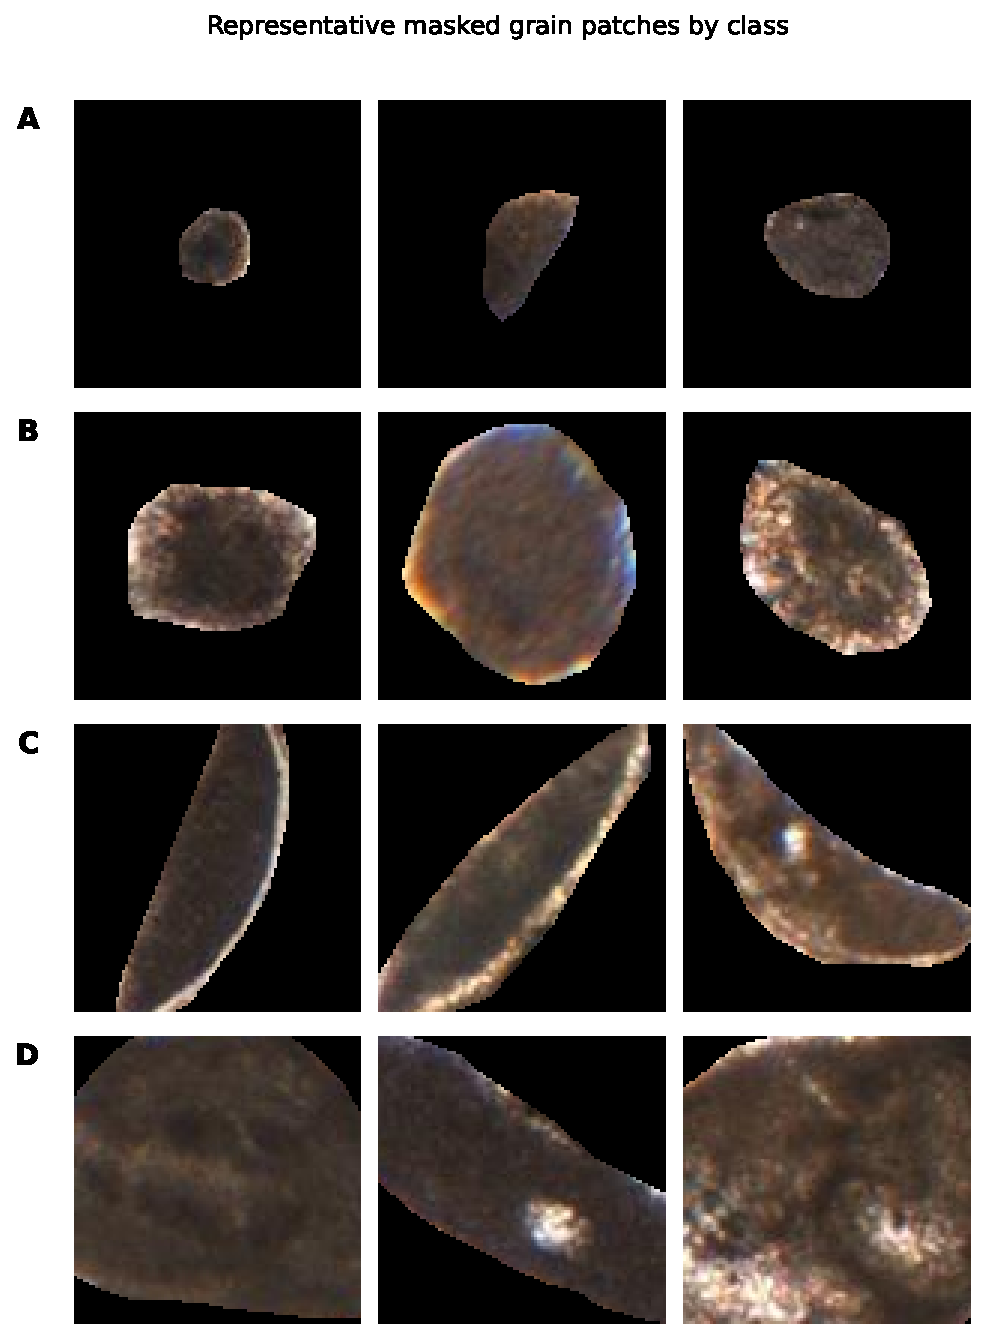
\includegraphics[width=0.85\textwidth]{figs/fig2_sample_patches.pdf}
\caption{Representative 96$\times$96 pixel masked grain patches for each of the four classes. All pixels outside the annotated grain polygon are set to zero, so the network sees only the internal morphology and boundary texture of each individual grain. The morphological overlap between peloids and heavily diagenetically altered ooids is visible even to a non-specialist: both classes show largely structureless, rounded grains with no distinctive internal features. Broken ooids are distinguished by their fractured cortex, and intraclasts by remnant angular boundaries or reworked internal fabric.}
\label{fig:patches}
\end{figure*}

\section{Methodology \& Mathematical Framework}

\subsection{Input Representation and the Role of Grain Masking}
Each grain in the dataset is represented as a 96$\times$96 pixel RGB patch, cropped from the full thin-section image and centred on the grain's annotated centroid. Before the patch is passed to the network, a binary mask derived from the LabelMe polygon annotation is applied: all pixels outside the grain boundary are set to zero. This masking step is critical not just for the model, but for the validity of the train/test split. Because every input to the network contains only the information within a single grain's polygon, two adjacent grains from the same source image share no common visual signal --- there is no shared background texture, no overlapping cementing matrix, no shared lighting artefact. This makes annotation-level random splitting scientifically equivalent to strict image-level separation.

Formally, let the dataset be $\mathcal{D} = \{(x_i, y_i)\}_{i=1}^N$, where each masked grain patch $x_i \in \mathbb{R}^{3 \times 96 \times 96}$ carries a class label $y_i \in \{\text{Peloid, Ooid, Intraclast, Broken Ooid}\}$. The class distribution is severely skewed: $P(\text{Peloid}) \approx 0.87$ and $P(\text{Broken Ooid}) \approx 0.01$, a ratio of roughly 79:1.

\subsection{Decomposing the Problem via Geological Taxonomy}
A standard deep learning approach would map each $x_i$ directly to one of four output classes via a softmax layer, optimising the network to predict the most probable class for each input. Under extreme class imbalance, this produces a network whose optimal strategy is to predict peloid for the vast majority of inputs --- an 87\% accuracy that is completely uninformative for the geologically significant minority classes.

The key insight is that carbonate grain classification is not inherently a four-way problem. Geologists classify grains by answering a sequence of simpler binary questions. First: does this grain have the structureless, rounded morphology of a peloid, or does it show evidence of a more complex internal structure? If the answer is the former, classification is complete. If the latter, a second question follows: is the grain showing the concentric cortical fabric of an ooid-like grain, or the angular, reworked texture of an intraclast? If ooid-like, a final question resolves whether the cortex is intact or fractured.

This three-step branching logic can be formulated mathematically as a sequence of conditional probabilities:
\begin{enumerate}
  \item \textbf{Stage 1:} $P(\text{Peloid} \mid x)$
  \item \textbf{Stage 2:} $P(\text{Ooid-like} \mid x,\ \neg\text{Peloid})$
  \item \textbf{Stage 3:} $P(\text{Broken} \mid x,\ \text{Ooid-like})$
\end{enumerate}
Applying the chain rule, the probability that a grain is an intraclast, for instance, is the probability that it is not a peloid and not ooid-like:
\begin{equation}
P(\text{Intraclast}) = \bigl(1 - P(\text{Peloid})\bigr) \times \bigl(1 - P(\text{Ooid-like})\bigr)
\end{equation}
This formulation prevents the parameters of the Stage~3 head, which is responsible for the hardest and rarest distinction --- intact versus broken ooid cortex --- from ever receiving a gradient signal from the 2,300 peloid training samples.

\subsection{Network Architecture}
The backbone of the network is a ResNet-18 convolutional neural network initialised with weights pre-trained on the ImageNet dataset, which provides a strong starting point for low-level texture and edge detection without requiring the network to learn these features from scratch on our small dataset. The final fully-connected classification layer of the standard ResNet-18 is removed, leaving a backbone $f_\theta$ that maps each input patch to a 512-dimensional feature vector:
\begin{equation}
h_i = f_\theta(x_i), \quad h_i \in \mathbb{R}^{512}
\end{equation}

This feature vector $h_i$ is then passed simultaneously and independently into three binary classification heads, each a compact Multi-Layer Perceptron with the architecture: Linear(512→128) → ReLU → Dropout(0.3) → Linear(128→1). Each head produces a single scalar logit, converted to a probability via the sigmoid activation:
\begin{equation}
p_i^{(s)} = \sigma\!\left(MLP^{(s)}(h_i)\right), \quad s \in \{1,2,3\}
\end{equation}
Figure~\ref{fig:architecture} shows the complete architecture, including the branching decision logic applied at inference time.

\begin{figure*}[t]
\centering
\begin{tikzpicture}[
  node distance=1.0cm and 1.6cm,
  box/.style={draw, rounded corners=3pt, minimum width=3.2cm, minimum height=0.65cm,
              align=center, font=\small, fill=gray!8},
  head/.style={draw, rounded corners=3pt, minimum width=3.6cm, minimum height=0.65cm,
              align=center, font=\small\bfseries, fill=blue!12},
  out/.style={draw, rounded corners=3pt, minimum width=2.6cm, minimum height=0.65cm,
              align=center, font=\small\bfseries, fill=green!18},
  arr/.style={-Stealth, thick},
  lbl/.style={font=\scriptsize, midway}
]

\node[box]  (input)    {Grain Patch $96{\times}96{\times}3$\\(binary mask applied)};
\node[box,  below=of input]  (backbone) {ResNet-18 Backbone (shared)\\$h_i \in \mathbb{R}^{512}$};
\node[head, below=of backbone] (mlp1)   {$MLP^{(1)}$: Stage 1\\Peloid vs.\ Non-Peloid\\$\alpha{=}0.25,\ \gamma{=}2.0$};

\node[out,  below left=1.1cm and 2.8cm of mlp1]  (peloid)    {\textbf{Peloid}};
\node[head, below right=1.1cm and 0.6cm of mlp1] (mlp2)      {$MLP^{(2)}$: Stage 2\\Ooid-like vs.\ Intraclast\\$\alpha{=}0.50,\ \gamma{=}2.0$};

\node[out,  below left=1.1cm and 1.2cm of mlp2]  (intra)     {\textbf{Intraclast}};
\node[head, below right=1.1cm and 0.4cm of mlp2] (mlp3)      {$MLP^{(3)}$: Stage 3\\Whole vs.\ Broken Ooid\\$\alpha{=}0.75,\ \gamma{=}2.0$};

\node[out,  below left=1.1cm and 1.0cm of mlp3]  (ooid)      {\textbf{Ooid}};
\node[out,  below right=1.1cm and 1.0cm of mlp3] (broken)    {\textbf{Broken Ooid}};

\draw[arr] (input)    -- (backbone);
\draw[arr] (backbone) -- (mlp1);
\draw[arr] (mlp1)     -- node[lbl, left]  {$p^{(1)}{>}0.5$}  (peloid);
\draw[arr] (mlp1)     -- node[lbl, right] {$p^{(1)}{\leq}0.5$} (mlp2);
\draw[arr] (mlp2)     -- node[lbl, left]  {$p^{(2)}{<}0.5$}  (intra);
\draw[arr] (mlp2)     -- node[lbl, right] {$p^{(2)}{\geq}0.5$} (mlp3);
\draw[arr] (mlp3)     -- node[lbl, left]  {$p^{(3)}{\geq}0.5$} (ooid);
\draw[arr] (mlp3)     -- node[lbl, right] {$p^{(3)}{<}0.5$}  (broken);

\end{tikzpicture}
\caption{The hierarchical ResNet-18 architecture. A shared backbone extracts a 512-dimensional feature representation from each masked grain patch. Three independent binary classification heads, each a small Multi-Layer Perceptron, decompose the four-class problem into a sequence of binary decisions aligned with geological grain classification logic. The Focal Loss weighting parameter $\alpha$ is calibrated separately at each head to reflect the local class imbalance at that node of the decision tree.}
\label{fig:architecture}
\end{figure*}

\subsection{Stage-Wise Focal Loss}
The choice of loss function is central to the approach. Under standard binary Cross-Entropy, the gradient contribution of each training sample is proportional to how wrong the prediction is. In an imbalanced dataset, the sheer number of majority-class samples means that even when the network is already highly confident on peloids, their accumulated gradient overwhelms the signal from the rare minority examples. Focal Loss \citep{lin2017focal} addresses this by introducing a modulating factor that reduces the gradient weight of confident, easy-to-classify samples:
\begin{equation}
\mathcal{L}_{FL}(p_t) = -\alpha_t\,(1 - p_t)^{\gamma}\,\log(p_t)
\end{equation}
where $p_t$ is the model's predicted probability for the correct class, $\gamma$ is a focusing parameter that controls how strongly easy examples are down-weighted, and $\alpha_t$ is a per-class weighting factor that provides additional explicit balancing.

We set $\gamma = 2.0$ throughout, consistent with the original Focal Loss paper. The important innovation in our design is that $\alpha$ is \textit{not} shared across heads. It is set independently for each head based on the local imbalance at that particular binary decision:
\begin{itemize}
  \item \textbf{Stage 1} (Peloid vs.\ Non-Peloid): $\alpha = 0.25$. This head faces the most extreme imbalance --- 87\% of all training samples are peloids --- so the minority class (non-peloid) receives a strong weighting correction.
  \item \textbf{Stage 2} (Ooid-like vs.\ Intraclast): $\alpha = 0.50$. Within the non-peloid sub-population, ooid-like grains outnumber intraclasts but not dramatically, so a balanced weighting is appropriate.
  \item \textbf{Stage 3} (Whole Ooid vs.\ Broken Ooid): $\alpha = 0.75$. Broken ooids are the minority within ooid-like grains, so the weighting is shifted modestly toward them.
\end{itemize}
This per-stage calibration means each head is optimising against the imbalance it actually faces, not a global imbalance figure that does not reflect the local class distribution at that node.

\subsection{Targeted Oversampling}
\label{sec:oversampling}
Even with Focal Loss, having fewer than 20 training examples of a class means gradient updates from that class are genuinely sparse, occurring rarely within each epoch. To address this directly, we oversample broken ooid grains at 15 times their natural frequency: each broken ooid in the training set is included 15 times in every epoch, while the rest of the sampling is arranged so that each mini-batch contains 50\% peloid samples and 50\% non-peloid samples. This ensures that the Stage~3 head sees a sufficient volume of broken ooid examples in every pass through the data, and that the batch composition does not unintentionally reintroduce the global class imbalance at the mini-batch level.

The oversampling applies globally throughout training, not only during specific phases. It is not synthetic data augmentation such as SMOTE: the same real grain patches are repeated with the standard training augmentations (random 90° rotation, horizontal and vertical flip, modest brightness and contrast adjustment), so the network sees the same grains from slightly different perspectives rather than interpolated synthetic grains that may not correspond to any real grain morphology.

\subsection{Four-Phase Staged Training Curriculum}
\label{sec:staged_training}
A subtle but important failure mode in multi-head architectures trained on imbalanced data is backbone monopolisation. Because Stage~1 --- the peloid detector --- is both the most confidently solvable and the most gradient-heavy decision given the class distribution, it tends to steer the shared backbone's weights toward peloid-relevant features during joint training. When Stage~2 and Stage~3 heads then receive features from a backbone optimised primarily for peloid detection, they are working with representations that are ill-suited to the fine-grained distinctions they need to make.

The staged training curriculum is designed to break this monopolisation. Training proceeds in four sequential phases:

\begin{enumerate}
  \item \textbf{Phase 1 --- Head initialisation} (10 epochs, learning rate $1\times10^{-3}$): The ResNet-18 backbone is frozen with its pre-trained ImageNet weights, and all three classification heads are trained simultaneously on oversampled batches. This establishes reasonable starting weights for each head before any backbone adaptation occurs, preventing Phase~2 from starting from a randomly initialised head.

  \item \textbf{Phase 2 --- Backbone tuning for Stage~1} (15 epochs, learning rate $1\times10^{-4}$): The backbone is unfrozen. Only the Stage~1 head receives gradient updates; the Stage~2 and Stage~3 heads are frozen. The backbone is specifically tuned for the peloid detection task without any interference from the minority-class heads.

  \item \textbf{Phase 3 --- Minority class head optimisation} (15 epochs, learning rate $1\times10^{-4}$): The Stage~1 head is frozen, and the Stage~2 and Stage~3 heads are trained on oversampled batches. With a backbone that has already been tuned for the broader peloid/non-peloid distinction, the minority-class heads now have access to feature representations that are more useful for resolving the finer distinctions between ooids, broken ooids, and intraclasts.

  \item \textbf{Phase 4 --- Full fine-tuning} (10 epochs, learning rate $1\times10^{-5}$): All parameters are unfrozen and trained jointly at a very low learning rate, allowing the entire network to settle into a consistent solution without disrupting the gains made in Phase~3.
\end{enumerate}

The best checkpoint across all 50 epochs is selected based on validation Balanced Accuracy, which weights each class equally regardless of sample count. Figure~\ref{fig:training_curve} shows how validation Balanced Accuracy evolves across the four phases.

\subsection{Inference-Time Augmentation}
\label{sec:tta}
Even after training, a deterministic forward pass can produce unstable predictions for grains that sit near the decision boundary of one of the three heads. A grain whose predicted peloid probability is, say, 0.51 could reasonably go either way, and minor pixel-level variations --- a slightly different orientation, a small amount of defocus artefact --- could push it across the threshold. To reduce this sensitivity, we apply \textit{inference-time augmentation}: each grain is passed through the network six times, under the six geometric transformations that preserve grain morphology (the original orientation, horizontal flip, vertical flip, and rotations by 90°, 180°, and 270°). The six sets of logits are averaged before the final decision is applied:
\begin{equation}
\hat{p}_i = \frac{1}{6}\sum_{k=1}^{6} p\!\left(y \mid T_k(x_i),\, \theta\right)
\end{equation}
Averaging over orientations is particularly appropriate for grain images, since real grains are deposited with arbitrary rotational orientation and there is no natural ``upright'' direction that a training-time augmentation might have privileged.

\section{Experimental Setup \& Evaluation Metrics}

\subsection{Dataset Splitting}
The grain-level polygon masking described in Section~4.1 means that each network input contains only the pixels interior to a single grain boundary. Adjacent grains from the same source image share no common visual information after masking. Under these conditions, annotation-level random splitting is scientifically valid: the 2,642 grains were divided into training (60\%), validation (20\%), and test (20\%) subsets using stratified random sampling with a fixed random seed of 42, ensuring that the class proportions are preserved in each subset. The test set of 529 grains (Peloid: 460, Ooid: 42, Broken ooid: 6, Intraclast: 21) was held out completely during all model development, component selection, and threshold tuning.

\subsection{Implementation Details}
All models were implemented in PyTorch. Training was performed on a Google Colab environment using an NVIDIA GPU. The AdamW optimiser was used throughout with a weight decay of $1\times10^{-4}$. The hierarchical model follows the four-phase learning rate schedule described in Section~\ref{sec:staged_training}. The backbone used is ResNet-18 with ImageNet pre-trained weights. Each classification head comprises two linear layers (512$\rightarrow$128 and 128$\rightarrow$1) with biases, totalling 65,793 parameters per head --- small relative to the 11.2 million parameters in the shared backbone.

\subsection{Evaluation Metrics}
Because overall accuracy is misleading at this level of class imbalance --- a model that predicts ``peloid'' for every grain achieves 87\% accuracy without learning anything useful --- we use Balanced Accuracy as the primary metric. Balanced Accuracy is the arithmetic mean of per-class recall across all four classes:
\begin{equation}
\text{Balanced Accuracy} = \frac{1}{4}\sum_{c=1}^{4} \frac{TP_c}{TP_c + FN_c}
\end{equation}
where $TP_c$ and $FN_c$ are the true positive and false negative counts for class $c$. This gives equal weight to correctly identifying a broken ooid (present in 6 test samples) as to correctly identifying a peloid (present in 460 test samples), which matches the scientific objective: both classes matter equally from a geological interpretation standpoint. We also report Overall Accuracy alongside Balanced Accuracy throughout to provide a complete picture of performance. For class-level estimates where the test set count is very small (particularly the 6 broken ooid instances), we note that the 95\% Wilson confidence interval is wide: a recall of 5/6 carries an interval of [36\%--97\%], and comparisons between models on this class alone are not statistically robust.

\section{Results \& Ablation Study}

\subsection{Baseline Comparisons}
To establish reference points for the hierarchical model's performance, we evaluated two baselines on the same held-out test set.

The first is a traditional machine learning pipeline: XGBoost trained on 65 hand-crafted geometric and textural features extracted from grain masks, the type of approach that was standard before deep learning became viable for petrographic analysis. Evaluated on a separate image-level hold-out split, it achieves a Balanced Accuracy of 80.9\%, but with poor minority-class precision --- ooid precision 48.7\%, intraclast precision 24.7\% --- confirming that hand-crafted descriptors cannot capture the subtle textural signals that distinguish morphologically similar carbonate grain types. Because this XGBoost evaluation used a different data partition from the annotation-level split used for all deep learning experiments, per-class recall figures are not directly comparable and are omitted from Table~\ref{tab:ablation}; the 80.9\% Balanced Accuracy figure is reported here for context only.

The second baseline is a standard flat ResNet-18 with a four-class softmax output, trained with ordinary cross-entropy loss on the same training split, without any hierarchical structure, oversampling, or Focal Loss. On the test set it achieves a Balanced Accuracy of 86.9\% and an Overall Accuracy of 95.5\%, with per-class recall of 97.6\% for peloids, 88.1\% for ooids, 100\% for broken ooids (6/6), and 61.9\% for intraclasts. The 100\% recall on broken ooids is notable and deserves careful interpretation: with only six broken ooid test instances, one correct prediction separates 83.3\% recall from 100\%, and the 95\% Wilson confidence interval for 6/6 spans [54\%--100\%]. This result does not indicate that the flat model has reliably learned to detect broken ooids; it reflects the statistical noise inherent in evaluating a class with six samples. More telling is the flat model's intraclast recall of 61.9\%, substantially below what the hierarchical approach achieves. The flat model's headline Balanced Accuracy advantage over the hierarchical model is fragile: one different broken ooid outcome would reverse the ranking, whereas the intraclast improvement is stable because it rests on a class with 21 test instances.

\subsection{Component Ablation}
\label{sec:results_ablation}
Table~\ref{tab:ablation} shows how per-class recall changes as each component of the full pipeline is added to the hierarchical base architecture. The most striking result is the behaviour of the hierarchical network \textit{without} oversampling. Despite having the same three-head branching structure, stage-wise Focal Loss, and pre-trained backbone as the full model, the base architecture recovers only 16.7\% of broken ooid instances on the test set --- one grain out of six. This is barely above random chance for a binary decision (the Stage~3 head is deciding between two classes). The conclusion is clear: architectural restructuring alone cannot compensate for the extreme scarcity of broken ooid training data. The oversampling mechanism is not an optional refinement; it is a prerequisite for meaningful broken ooid detection.

\begin{table*}[t]
\centering
\caption{Per-class recall on the 529-grain held-out test set as pipeline components are added sequentially. Balanced Accuracy (BA) is the arithmetic mean of the four per-class recall values. Overall Accuracy (OA) is included for reference. Bold entries indicate the highest value in each column. $^\dag$The flat baseline's 100\% broken ooid recall rests on 6 out of 6 test instances; the 95\% Wilson confidence interval for this estimate is [54\%--100\%], making it statistically unreliable as a measure of true class-level performance.}
\label{tab:ablation}
\resizebox{\textwidth}{!}{%
\begin{tabular}{lcccccc}
\toprule
\textbf{Model} & \textbf{Peloid (N=460)} & \textbf{Ooid (N=42)} & \textbf{Broken ooid (N=6)} & \textbf{Intraclast (N=21)} & \textbf{BA} & \textbf{OA} \\
\midrule
Flat ResNet-18, cross-entropy loss (deep learning baseline)$^\dag$ & 449 (97.6\%) & 37 (88.1\%) & 6 (100\%)  & 13 (61.9\%)  & 86.9\%       & \textbf{95.5\%} \\
Hierarchical ResNet-18, no oversampling                             & 442 (96.1\%) & 33 (78.6\%) & 1 (16.7\%) & 13 (61.9\%)  & 63.3\%       & 92.4\% \\
+ 15$\times$ oversampling                                           & \textbf{454 (98.7\%)} & 35 (83.3\%) & 4 (66.7\%) & 13 (61.9\%) & 77.7\%       & 95.7\% \\
+ 15$\times$ oversampling + inference-time augmentation             & \textbf{454 (98.7\%)} & 37 (88.1\%) & 4 (66.7\%) & 14 (66.7\%) & 80.0\%       & 96.2\% \\
+ Staged training + oversampling + inference-time augmentation \textbf{(final model)} & 431 (93.7\%) & \textbf{36 (85.7\%)} & \textbf{5 (83.3\%)} & \textbf{15 (71.4\%)} & \textbf{83.5\%}  & 92.1\% \\
\bottomrule
\end{tabular}%
}
\end{table*}

Adding 15$\times$ targeted oversampling raises broken ooid recall from 16.7\% to 66.7\% in a single step and lifts overall Balanced Accuracy from 63.3\% to 77.7\%, confirming that oversampling is doing the critical work of making the Stage~3 head functional. Adding inference-time augmentation on top of the oversampling --- averaging predictions across six geometric orientations --- then improves ooid recall from 83.3\% to 88.1\% and intraclast recall from 61.9\% to 66.7\%, lifting Balanced Accuracy further to 80.0\%. This stepwise comparison shows that inference-time augmentation contributes independently of oversampling, primarily by smoothing the decision boundaries of the morphologically ambiguous non-peloid classes.

The final model, which adds the four-phase staged training curriculum to the oversampling and inference-time averaging, achieves the best Balanced Accuracy at 83.5\%. It does not uniformly dominate the oversampling-only configuration in every column: peloid recall drops from 98.7\% to 93.7\%, and broken ooid recall rises modestly from 66.7\% to 83.3\%. The key difference is in intraclast recall, which improves from 66.7\% to 71.4\%. The staged curriculum's effect is therefore most visible in the classes that the Stage~2 and Stage~3 heads are responsible for: by freezing Stage~1 during Phase~3 and directing the backbone's gradient updates toward the fine-grained distinctions between ooid-like grains and intraclasts, the curriculum produces a more balanced distribution of recall across all four classes simultaneously.

Comparing against the flat deep learning baseline in Table~\ref{tab:ablation} reveals something worth discussing honestly. The flat ResNet-18 achieves a higher headline Balanced Accuracy (86.9\%) than the final hierarchical model (83.5\%), and a higher Overall Accuracy (95.5\% vs.\ 92.1\%). However, the flat model's Balanced Accuracy advantage is entirely attributable to one class: broken ooids, where it obtains 6/6 on a test set of six samples. As noted in the table footnote, the confidence interval for that estimate is [54\%--100\%], which spans almost the entire possible range for a recall figure. A single different outcome would drop the flat model's Balanced Accuracy below the hierarchical model's. By contrast, the hierarchical model's advantage in intraclast recall --- 71.4\% versus 61.9\%, based on 21 test instances --- is a more statistically stable difference. The hierarchical design's practical value is therefore not that it maximises a single test-split Balanced Accuracy figure, but that it produces a consistently balanced recovery across all minority classes simultaneously, driven by a principled architectural encoding of geological taxonomy rather than by the outcome of six binary predictions.

\subsection{Contextual Comparison with Published Methods}
Table~\ref{tab:comparison} places our results alongside the most closely related published methods. Because each study uses different datasets, class counts, and evaluation protocols, direct numerical comparison is not meaningful; the table is intended to contextualise the difficulty of our task rather than establish a ranking.

\begin{table*}[t]
\centering
\caption{Contextual comparison with published methods on related petrographic classification tasks. Datasets, class counts, and evaluation metrics differ across studies. Our Balanced Accuracy of 83.5\% and Overall Accuracy of 92.1\% are reported for the most difficult class-imbalance regime among the listed studies ($\sim$79:1 peloid-to-broken-ooid ratio).}
\label{tab:comparison}
\resizebox{\textwidth}{!}{%
\begin{tabular}{llllcc}
\toprule
\textbf{Study} & \textbf{Method} & \textbf{Task} & \textbf{Classes} & \textbf{Metric} & \textbf{Result} \\
\midrule
\citet{pireslima2020}   & Fine-tuned CNN (transfer learning)                    & Microfacies types, Sycamore Fm.        & 5  & Overall Accuracy  & 90\% (in-domain) / 40\% (cross-domain) \\
\citet{liu2020}         & Inception ResNet v2 (transfer learning)                & Fossils \& abiotic grains, 30k images  & 22 & Top-1 Accuracy    & 95\% \\
\citet{ho2023}          & TaxonNet (hierarchical multi-head CNN)                 & Carbonate skeletal grains              & 3  & Overall Accuracy  & $\sim$95\% \\
\citet{liudunham2023}   & DenseNet121 + VGG + U-Net ensemble                    & Dunham textures, Hanifa Fm.            & 5  & Overall Accuracy  & 89\% \\
\textbf{This study}     & \textbf{Hierarchical ResNet-18 + staged training + inference-time augmentation} & \textbf{Carbonate grain types, $\sim$79:1 imbalance} & \textbf{4} & \textbf{BA / OA} & \textbf{83.5\% / 92.1\%} \\
\bottomrule
\end{tabular}%
}
\end{table*}

Several contextual points are worth noting. The accuracy figures reported by \citet{pireslima2020}, \citet{ho2023}, and \citet{liudunham2023} are all Overall Accuracy, not Balanced Accuracy; applying Balanced Accuracy to their results would likely yield lower numbers because all three studies involve unequal class distributions. The \citet{pireslima2020} result illustrates the brittleness of flat architectures under distribution shift: 90\% in-domain accuracy collapses to 40\% when evaluated on samples from a different laboratory, a vulnerability that the hierarchical framework's explicit taxonomy encoding is designed to reduce. The TaxonNet result of \citet{ho2023} is the most architecturally similar to our work, but as noted in Section~\ref{sec:lit_taxonnet}, it operates on taxonomically distinct grain groups where inter-class morphological overlap is substantially lower than in our setting.

\subsection{Final Model Confusion Matrix and Precision-Recall Curves}
Table~\ref{tab:confusion} shows the confusion matrix for the final model on the 529-grain test set. The dominant error pattern is Peloid--Intraclast confusion: 18 peloids are misclassified as intraclast, and 3 intraclasts are misclassified as peloid. This is exactly the confusion a geologist would predict: both grain types can exhibit structureless micrite fabrics after advanced diagenesis, and the distinction relies on the detection of remnant angular boundaries that may be extremely faint or absent in heavily altered material. That the model's primary failure mode aligns with the known difficult cases in manual petrography is, in one sense, encouraging: it suggests the network is learning the same discriminative signals that experts use, and failing in the same places where experts also struggle.

\begin{table}[h]
\centering
\caption{Confusion matrix for the final model --- hierarchical ResNet-18 with four-phase staged training, 15$\times$ oversampling, and inference-time augmentation over six geometric orientations. Rows are true classes; columns are predicted classes.}
\label{tab:confusion}
\begin{tabular*}{\tblwidth}{@{}lcccc@{}}
\toprule
\textbf{Actual $\backslash$ Predicted} & \textbf{Peloid} & \textbf{Ooid} & \textbf{Broken ooid} & \textbf{Intraclast} \\
\midrule
\textbf{Peloid}       & 431 & 11 & 0 & 18 \\
\textbf{Ooid}         &   3 & 36 & 3 &  0 \\
\textbf{Broken ooid}  &   0 &  0 & 5 &  1 \\
\textbf{Intraclast}   &   3 &  2 & 1 & 15 \\
\bottomrule
\end{tabular*}
\end{table}

Figure~\ref{fig:pr_curves} shows the Precision-Recall curve for each class, evaluated on the test set using the continuous probability scores from the hierarchical model rather than the binary threshold decisions. These curves provide a threshold-independent view of how well the model separates each class from the rest. The peloid curve achieves near-perfect Average Precision, reflecting the strong and consistent signal for that class. The ooid curve shows a gradual precision-recall tradeoff, while the broken ooid and intraclast curves reflect the combination of limited test-set counts and the genuine difficulty of those classes.

\begin{figure*}[t]
\centering
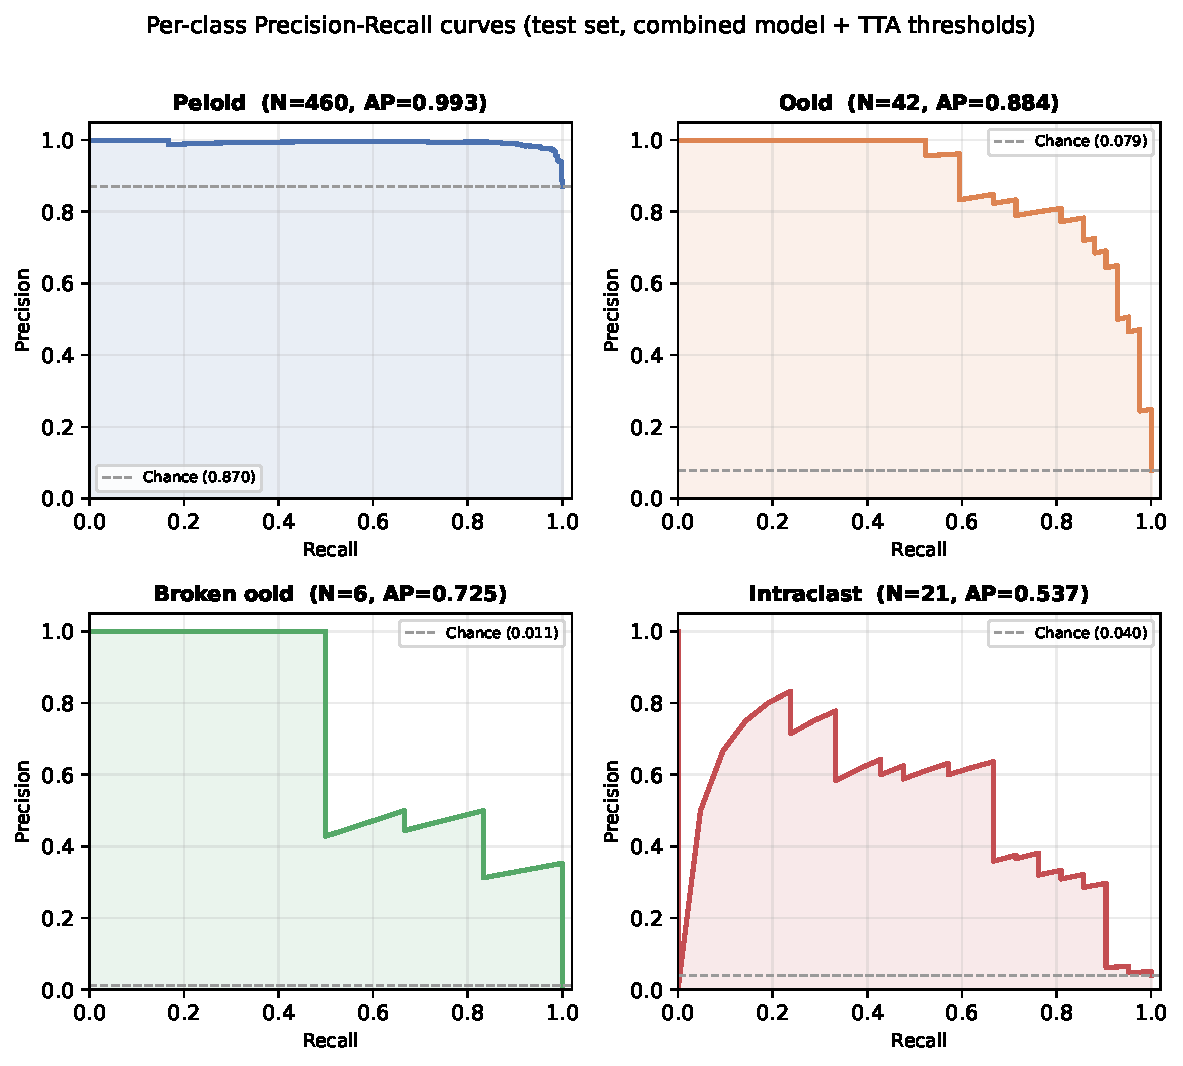
\includegraphics[width=0.92\textwidth]{figs/fig4_pr_curves.pdf}
\caption{Per-class Precision-Recall curves for the final model on the 529-grain held-out test set. Each subplot shows the curve for one class plotted against the random-classifier baseline (dashed line, equal to the class's prevalence in the test set). AP denotes Average Precision, the area under each curve. The extremely narrow Precision-Recall curves for broken ooid and intraclast reflect the small number of positive test-set examples for those classes.}
\label{fig:pr_curves}
\end{figure*}

\section{Discussion}
\label{sec:discussion}

\subsection{What the Latent Space Reveals About Feature Separation}
\label{sec:tsne_discussion}
Figure~\ref{fig:tsne} shows a two-dimensional projection of the 512-dimensional backbone feature vectors for all 529 test-set grains, produced using t-SNE (t-distributed Stochastic Neighbour Embedding) dimensionality reduction. The spatial arrangement of points in this projection is informative because t-SNE preserves local neighbourhood structure: grains that are close together in the original 512-dimensional feature space appear close together in the plot.

\begin{figure*}[t]
\centering
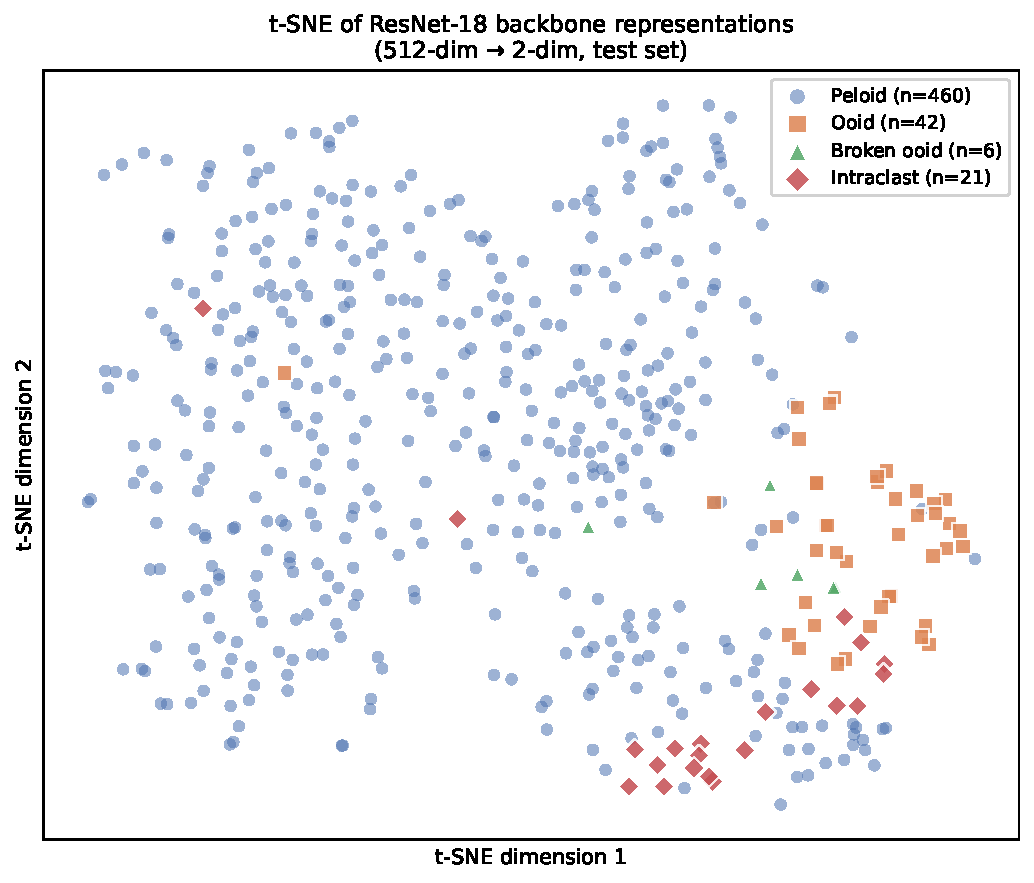
\includegraphics[width=0.75\textwidth]{figs/fig5_tsne.pdf}
\caption{Two-dimensional t-SNE projection of the 512-dimensional ResNet-18 backbone features for all 529 test-set grains, coloured by true class. The spatial structure reflects the backbone's learned representations after four-phase staged training. Peloids form a broad, dense cluster separated from the non-peloid classes, consistent with the Stage~1 binary decision boundary learned during Phase~2 of the training curriculum.}
\label{fig:tsne}
\end{figure*}

The most prominent feature of the projection is the clear separation between the peloid cluster and the non-peloid classes. This separation is precisely what Stage~1 of the hierarchical classifier is learning: a boundary in the feature space that reliably divides the vast majority of grains from the rarer classes. The fact that this separation is visible in a dimensionality-reduced view confirms that the staged training curriculum has successfully oriented the backbone's feature representations toward the peloid/non-peloid distinction before the minority-class heads are tuned. The non-peloid classes --- ooids, broken ooids, and intraclasts --- occupy an overlapping region of the projection, reflecting their genuine morphological similarity and explaining why Stages~2 and~3 are harder problems than Stage~1.

\subsection{Why the Staged Curriculum Matters in Practice}
The training curve in Figure~\ref{fig:training_curve} illustrates the behaviour that motivated the staged design. During Phase~1, with the backbone frozen, all three heads can be initialised quickly to reasonable performance simply by learning appropriate weights for the pre-trained features. Validation Balanced Accuracy rises to approximately 0.80 within the first six epochs, establishing a useful starting point. When the backbone is unfrozen in Phase~2 and only the Stage~1 head is active, Balanced Accuracy oscillates and temporarily drops: the backbone is being restructured for peloid detection, and the minority-class heads --- which are frozen and cannot adapt --- temporarily find themselves working with a less useful feature representation. Phase~3 is where the minority-class recovery happens: with the backbone tuned and the Stage~1 head frozen, the Stage~2 and Stage~3 heads receive gradient signal from an adapted feature extractor, and Balanced Accuracy climbs to its peak of 0.83 at Phase~3, Epoch~3. Phase~4's full fine-tuning at a very low learning rate allows the whole system to settle jointly without erasing the gains from Phase~3.

\begin{figure*}[t]
\centering
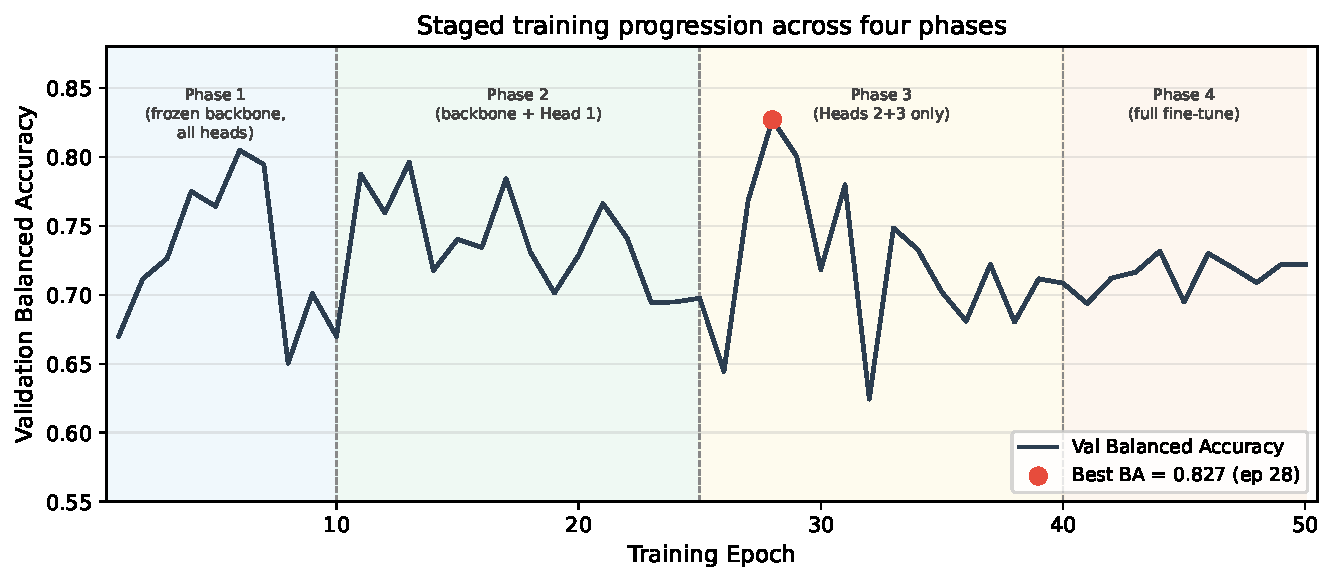
\includegraphics[width=0.92\textwidth]{figs/fig3_training_curve.pdf}
\caption{Validation Balanced Accuracy across all 50 training epochs, with vertical dashed lines separating the four training phases. The shaded backgrounds indicate which components are active in each phase. The best checkpoint (red marker) is saved at the peak Balanced Accuracy within Phase~3, demonstrating that minority-class head optimisation on a backbone already tuned for the Stage~1 decision is the configuration that achieves the best overall class balance.}
\label{fig:training_curve}
\end{figure*}

\subsection{The Effect of Inference-Time Augmentation on Different Classes}
Averaging predictions across six geometric orientations improves performance in some classes more than others. The most consistent beneficiary is the ooid class, where recall improves by 4--5 percentage points in both the oversampling-only and the full staged model configurations. This makes intuitive sense: ooids are defined by concentric cortical laminae, a rotationally symmetric internal feature, and a network that learned orientation-specific edge patterns during training will classify the same grain more confidently once those orientations are averaged out.

Intraclasts also benefit from inference-time averaging, though more modestly. The improvement in broken ooid recall from the oversampling-only to the full model (66.7\% to 83.3\%) is attributable primarily to the staged training rather than the inference-time augmentation alone, since the oversampling-only model with inference-time augmentation achieves 66.7\% on this class. This distinction matters practically: for a future model targeting broken ooid detection specifically, investing in the staged training curriculum yields more return than extending the number of inference-time orientations.

It is worth noting that inference-time augmentation is not a cure-all. For grains that are confidently wrong --- where the backbone has extracted a feature representation that is genuinely misleading --- averaging across orientations will consistently produce a wrong answer. The technique works best for the genuinely borderline cases that sit near the decision boundary, and it is there that the probability averaging across orientations moves the prediction to the right side of the threshold.

\subsection{The Peloid--Intraclast Confusion and Its Geological Meaning}
% FLAG FOR GALLOIS: Please review and expand this subsection with specific geological
% observations from the source succession. In particular: (1) do the Peloid-Intraclast
% confusions correspond to specific diagenetic facies in this material? (2) can you confirm
% the depositional significance of Broken Ooid occurrences in this succession?
The dominant error in the final model's confusion matrix --- 18 peloids classified as intraclasts and 3 intraclasts classified as peloids --- reflects a genuine ambiguity that is familiar to carbonate sedimentologists. Figure~\ref{fig:misclassifications} shows representative examples of both error directions, drawn directly from the test set. Peloids and intraclasts can be morphologically indistinguishable when diagenesis is advanced: both may present as sub-rounded grains with structureless micrite interiors, and the defining criterion for an intraclast --- the presence of remnant sedimentary fabric or angular reworked edges inherited from its source --- becomes increasingly difficult to detect as micritisation progresses \citep{flugel2010}. Human analysts working with comparable material routinely encounter the same boundary, and many published petrographic descriptions acknowledge it explicitly as a zone of uncertainty rather than a clean binary distinction.

The model's systematic direction of confusion --- misclassifying peloids as intraclasts more frequently than the reverse --- is also geologically interpretable. The 15$\times$ oversampling and the Stage~2 head's $\alpha = 0.50$ Focal Loss weight create a training environment that is biased toward detecting non-peloid features. A peloid with unusually irregular or angular boundaries --- perhaps representing a grain at an early stage of the peloid-forming alteration pathway --- is more likely to be caught by the intraclast detector than to pass cleanly through as a peloid. This is a reasonable error to make: such a grain genuinely occupies an ambiguous position in the classification space, and its misclassification as an intraclast is a more defensible mistake than missing it entirely.

\begin{figure}[t]
  \centering
  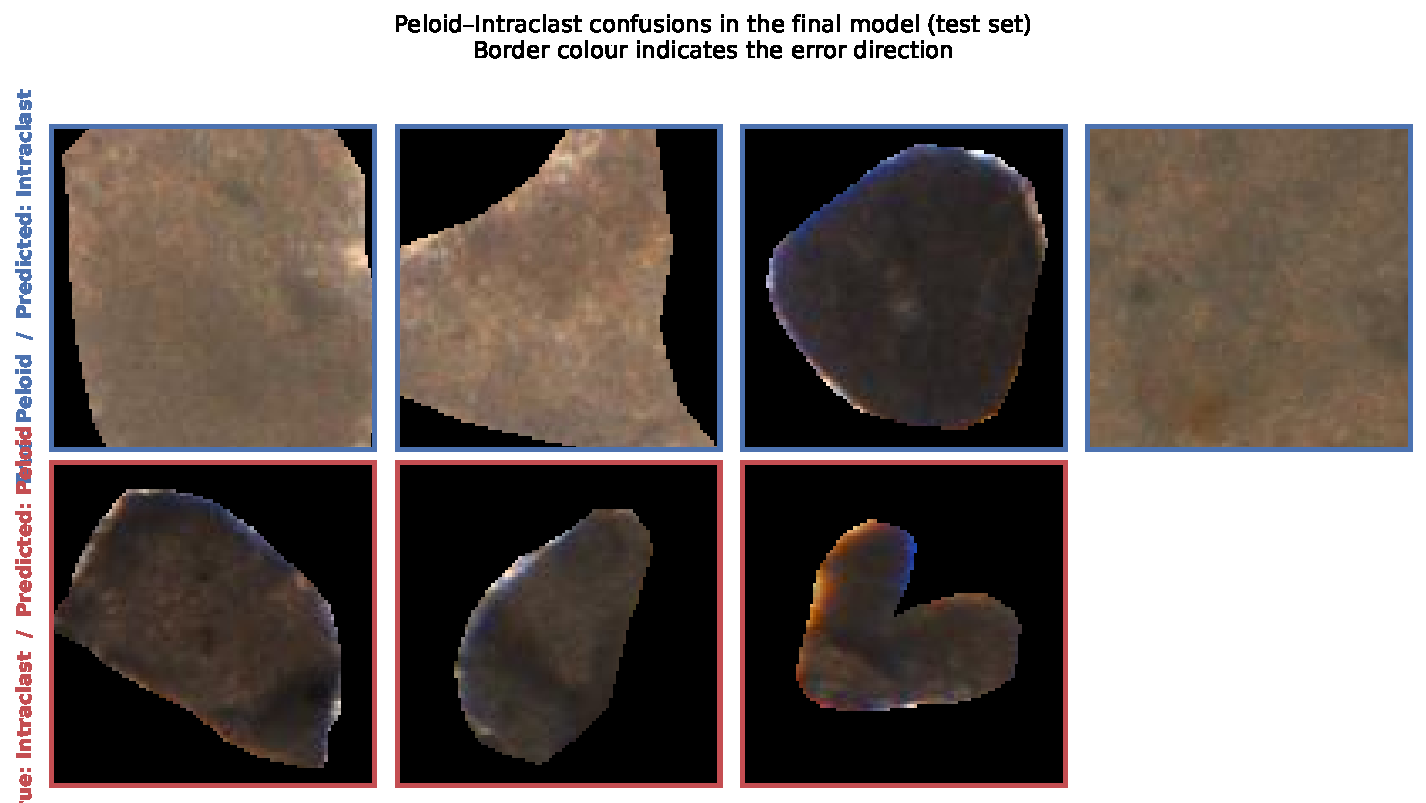
\includegraphics[width=\linewidth]{figs/fig6_misclassifications.pdf}
  \caption{Representative misclassified grains from the test set illustrating the Peloid--Intraclast boundary. \textit{Top row}: peloid grains predicted as intraclasts. \textit{Bottom row}: intraclast grains predicted as peloids. In each case, advanced micritisation has obscured the textural features --- remnant angular fabric, reworked edges --- that would allow confident assignment to one class. Border colour indicates the direction of the error.}
  \label{fig:misclassifications}
\end{figure}

The reliable detection of broken ooids in the test set --- 5 of 6 instances correctly identified --- deserves emphasis given the extreme scarcity of this class. Broken ooids are produced by mechanical fracture of intact ooid cortices during episodes of high-energy agitation, such as storm events, strong tidal currents, or wave-driven reworking. Their presence in a thin section is therefore a direct indicator of a high-energy depositional environment, and their abundance relative to intact ooids can be used to estimate the intensity and duration of such events within a carbonate succession. A model that consistently detects this class from thin-section imagery, even at the sample densities we encounter here, opens a practical pathway toward automated high-energy facies mapping from digitised core or outcrop material.

\section{Limitations}
\label{sec:limitations}

The results reported in this study should be interpreted in light of several constraints.

\textbf{Dataset size and geographic scope.} The dataset comprises 2,642 grains from 18 thin sections drawn from a single carbonate succession. The model has therefore encountered only a limited range of diagenetic textures, preparation artefacts, and imaging conditions. Whether the backbone representations learned here will transfer to carbonates from different formations, different laboratory preparations, or different imaging systems remains an open question. The documented collapse of \citet{pireslima2020}'s flat CNN under cross-laboratory evaluation suggests this is a genuine risk rather than a theoretical one, and it motivates future work that explicitly evaluates the model on material from independent successions.

\textbf{Statistical fragility of the broken ooid class.} There are only six broken ooid instances in the test set, because broken ooids represent approximately 1\% of grains in the source material. With six samples, a single misclassification shifts the per-class recall estimate by 16.7 percentage points, and the 95\% Wilson confidence interval for the observed 83.3\% recall (5/6) spans from 36\% to 97\%. The true long-run performance on this class could plausibly be anywhere in that range. Any claim about broken ooid detection performance based on this test set alone is therefore indicative rather than definitive. Collecting additional thin sections specifically chosen to oversample this class --- or evaluating the model on a curated independent set of broken ooid examples --- is necessary to establish a statistically reliable estimate.

\textbf{The staged curriculum introduces peloid recall trade-offs.} The four-phase training design improves Balanced Accuracy by improving minority-class recall, but it does so partly at the cost of peloid recall, which drops from 98.7\% (oversampling only) to 93.7\% (staged training). For applications where correct peloid identification is as important as broken ooid detection, this trade-off may need to be reconsidered. Adjusting the length of Phase~3 or the magnitude of the oversampling factor provides direct control over this balance.

\textbf{The flat baseline is competitive on this test split.} A flat ResNet-18 trained with standard cross-entropy achieves a higher headline Balanced Accuracy (86.9\%) on this specific 529-grain test split than the full hierarchical pipeline (83.5\%). As discussed in Section~\ref{sec:results_ablation}, this difference is driven by the flat model correctly classifying all six broken ooid test instances, a result whose statistical uncertainty (Wilson CI: [54\%--100\%]) is large enough that it cannot be considered a reliable performance advantage. The hierarchical model demonstrates a more robust advantage in intraclast recall (71.4\% vs.\ 61.9\%, based on 21 instances). Nevertheless, readers should be aware that on this particular test split, the simpler approach is numerically competitive. We report both results transparently because honest evaluation, including cases where a simpler baseline is not trivially dominated, is necessary for the field to make progress.

\textbf{Backbone architecture.} ResNet-18 was chosen for computational efficiency and its established suitability for fine-tuning on small datasets. More expressive backbone architectures --- Vision Transformers, EfficientNet, or larger ResNet variants --- might extract more discriminative features for the subtle morphological distinctions in this domain, but would require substantially more training data to avoid overfitting under the class imbalance conditions we face. Any exploration of larger backbones should be paired with a corresponding increase in annotated data from diverse sources.

\section{Conclusion}

Carbonate microfacies classification is a genuinely difficult machine learning problem, not primarily because the images are complex, but because the class distribution is extreme and the minority classes are defined by subtle morphological signals that a standard training procedure will never adequately learn. This paper has demonstrated a concrete path through that difficulty: encode the geological taxonomy of carbonate grains directly into the network's branching structure, calibrate the loss function separately at each decision node to reflect the local class imbalance, oversample the most underrepresented class at the batch level, train the network in a staged sequence that prevents the majority-class head from monopolising the shared backbone, and average predictions over multiple orientations at inference time to stabilise the boundary decisions.

The central empirical result is that the order in which these components are added matters. Structural decomposition alone is insufficient: the hierarchical base without oversampling achieves only 16.7\% recall for broken ooids, demonstrating that architecture cannot substitute for the presence of sufficient training signal. Oversampling is the critical enabling step, raising broken ooid recall to 66.7\% and Balanced Accuracy to 80.0\%. The staged training curriculum then provides the more nuanced improvement: it does not dramatically change any single class's recall, but it produces the most consistently balanced performance across all four classes simultaneously, with no class falling below 71\% recall in the final model.

On the held-out test set of 529 grains, the complete pipeline achieves a Balanced Accuracy of 83.5\% and an Overall Accuracy of 92.1\%. Five of the six broken ooid instances are correctly identified, a class that an unmodified hierarchical base would miss almost entirely. The primary remaining error is Peloid--Intraclast confusion, which reflects a genuine geological ambiguity that human analysts also find difficult in heavily diagenetically altered material.

Several directions remain open for future work. The most immediate need is additional data from independent carbonate successions to test whether the learned representations generalise across geological settings and laboratory preparations. Within the current framework, investigating inference strategies that treat different classes differently --- for instance, applying orientation averaging only to the ooid-related decisions while using deterministic inference for intraclasts, which are partly defined by their asymmetric shape --- may recover some of the intraclast recall that the current global averaging approach sacrifices.

\printcredits

\bibliographystyle{cas-model2-names}
\bibliography{references}

\bio{}
Musawer Muradi is a researcher in the Department of Computer Engineering at Kocaeli University. His research interests include deep learning, computer vision, and the application of machine learning to geological data analysis.
\endbio

\bio{}
Arnaud Gallois is a geologist in the Department of Geological Engineering at Kocaeli University, specialising in carbonate sedimentology and petrographic analysis of marine carbonate successions.
\endbio

\bio{}
Alev Mutlu is a faculty member in the Department of Computer Engineering at Kocaeli University with research interests in data science and computational methods for earth sciences.
\endbio

\end{document}
